\documentclass[letterpaper,12pt]{article}

%% Language and font encodings
\usepackage[english]{babel}

%% page size and margins (changable)
% \setlength{\evensidemargin}{0in}
% \setlength{\oddsidemargin}{0.5in}
% \setlength{\textwidth}{6in}
% \setlength{\topmargin}{0.2in}
% \setlength{\textheight}{8.6in}
% \setlength{\footnotesep}{14pt}
\usepackage[letterpaper,top=2cm,bottom=2cm,left=2cm,right=2cm,marginparwidth=1.75cm]{geometry}
\setlength {\marginparwidth}{2cm}

%% packages
\usepackage{amsmath,amsthm,amssymb,amsfonts}

% theorem types
\newtheorem{theorem}{Theorem}[section]
\newtheorem{lemma}[theorem]{Lemma}
\newtheorem{corollary}[theorem]{Corollary}
\newtheorem{conjecture}[theorem]{Conjecture}
\newtheorem{proposition}[theorem]{Proposition}
\newtheorem*{uconj}{Uniform Boundedness Conjecture}
\theoremstyle{definition}
\newtheorem{definition} [theorem] {Definition}
\newtheorem{claim}[theorem]{Claim}
\newtheorem{example} [theorem] {Example}
\newtheorem{remark} [theorem] {Remark}

\mathchardef\mhyphen="2D
\usepackage{graphicx}
\usepackage{tabularx}
\usepackage{array}
\usepackage[colorinlistoftodos]{todonotes}
\usepackage[colorlinks=true, allcolors=blue]{hyperref}
\usepackage{enumitem}
\usepackage{marginnote}
\usepackage{mathtools}
\usepackage[normalem]{ulem}
\usepackage[utf8]{inputenc}
\usepackage{fancyhdr}
\usepackage{booktabs}
\usepackage{enumitem}

\usepackage{pgfplots}
\pgfplotsset{compat=1.15}
\usepackage{mathrsfs}
\usetikzlibrary{arrows}

% user-defined macros
\newcommand{\C}{{\mathbb{C}}}
\newcommand{\F}{{\mathbb{F}}}
\newcommand{\N}{{\mathbb{N}}}
\newcommand{\Q}{{\mathbb{Q}}}
\newcommand{\PP}{{\mathbb{P}}}
\newcommand{\R}{{\mathbb{R}}}
\newcommand{\Z}{{\mathbb{Z}}}

\newcommand{\cK}{{\mathcal{K}}}

\newcommand{\fm}{{\mathfrak{m}}}
\newcommand{\fo}{{\mathfrak{o}}}

\newcommand{\Cp}{\C_p}
\newcommand{\Cv}{\C_v}
\newcommand{\Qp}{\Q_p}
\newcommand{\Qpbar}{\bar{\Q}_p}
\newcommand{\Dbar}{\overline{D}}

% user-defined math operators
\DeclareMathOperator{\rad}{rad}
\DeclareMathOperator{\diam}{diam}
\DeclareMathOperator{\divop}{div}

\begin{document}

\begin{titlepage}

 \begin{center}

  \vspace*{\fill}

  \vspace*{0.5cm}

  \huge\bfseries Midpoint and Trapezoidal Project

  \vspace*{0.5cm}

  \large{Henry Yu, Joseph Keeler, Kevin Ma}

  \vspace*{\fill}

 \end{center}

\end{titlepage}

\newpage

\section{Table of Values}

\begin{table}[h]
 \renewcommand*{\arraystretch}{1.8}
 \scalebox{1.1}{
  \hspace{-1cm}\begin{tabular}{|l|l|l|l|l|l|l|}
   \hline
   $f(x)$                     & $[a,b]$ & N    & M              & T             & E                 & $\dfrac{E-T}{E-M}$ \\
   \hline
   $f(x)=2x^{3}-5x^{2}+6$     & $[0,1]$ & $20$ & $4.83375$      & $4.8325$      & $4.8\overline{3}$ & $-1.999976$        \\
   \hline
   $f(x)=3x^{4}-x^{3}+7x$     & $[0,1]$ & $20$ & $3.849063047$  & $3.851874375$ & $3.85$            & $-2.0000500559$    \\
   \hline
   $sin(\frac{\pi x^{2}}{9})$ & $[0,1]$ & $20$ & $0.1152781773$ & $0.115483$    & $0.1153465199$    & $-1.996998944$     \\
   \hline
   $e^{2x}$                   & $[0,1]$ & $20$ & $3.193197384$  & $3.197189713$ & $3.194528049$     & $-2.000251002$     \\
   \hline
   $\sqrt{x+1}$               & $[0,1]$ & $20$ & $1.218966669$  & $1.21892091$  & $1.218951416$     & $-2.0$             \\
   \hline
  \end{tabular}}
\end{table}

\pagebreak

\section{Sides on the Integral}

\raggedright

\begin{large}

 Based on your table, are the midpoint and trapezoid approximations generally on the same side of the exact value of the integral? Justify your answer.

\end{large}

\vspace{1cm}

\begin{minipage}{0.45\textwidth}
 \begin{center}
  Midpoint and Exact
  \vskip 16pt
  \mbox{$4.83375>4.8\overline{3}\hspace{1cm}(M>E)$}
  \vskip 16pt
  \mbox{$3.849063047<3.85\hspace{1cm}(M<E)$}
  \vskip 16pt
  \mbox{$0.1152781773<0.1153465199\hspace{1cm}(M<E)$}
  \vskip 16pt
  \mbox{$3.193197384<3.194528049\hspace{1cm}(M<E)$}
  \vskip 16pt
  \mbox{$1.218966669>1.218951416\hspace{1cm}(M>E)$}
 \end{center}
\end{minipage}
\hfill
\begin{minipage}{0.45\textwidth}
 \begin{center}
  Trapezoid and Exact
  \vskip 16pt
  $4.8325<4.8\overline{3}\hspace{1cm}(T<E)$
  \vskip 16pt
  $3.851874375>3.85\hspace{1cm}(T>E)$
  \vskip 16pt
  $0.115483>0.1153465199\hspace{1cm}(T>E)$
  \vskip 16pt
  $3.197189713>3.194528049\hspace{1cm}(T>E)$
  \vskip 16pt
  $1.21892091<1.218951416\hspace{1cm}(T<E)$
 \end{center}
\end{minipage}

\vspace{1cm}

Based on the information presented, the midpoint and trapezoidal approximations are never on the same side.

\newpage

\section{Approximation Accuracy}

\begin{large}

 Which of the approximations, midpoint or trapezoidal, is generally closer to the exact value of the integral?

\end{large}

\vspace{1cm}

\Large\centerline{$\delta\hspace{0.1cm}(\%)=\dfrac{x_{estimate}-x_{actual}}{x_{actual}}$}
\normalsize

\vspace{0.7cm}
\centerline{Percent Error Formula}

\vspace{1cm}

\begin{minipage}{0.45\textwidth}
 \begin{center}
  Midpoint and Exact
  \vskip 16pt
  $\delta=0.008621\%$
  \vskip 16pt
  $\delta=0.024336\%$
  \vskip 16pt
  $\delta=0.059250\%$
  \vskip 16pt
  $\delta=0.041655\%$
  \vskip 16pt
  $\delta=0.001251\%$
  \vskip 16pt
  $\%\hspace{0.1cm}\text{avg}=0.0270226\%$
 \end{center}
\end{minipage}
\hfill
\begin{minipage}{0.45\textwidth}
 \begin{center}
  Trapezoid and Exact
  \vskip 16pt
  $\delta=0.017241\%$
  \vskip 16pt
  $\delta=0.048685\%$
  \vskip 16pt
  $\delta=0.118322\%$
  \vskip 16pt
  $\delta=0.083319\%$
  \vskip 16pt
  $\delta=0.002503\%$
  \vskip 16pt
  $\%\hspace{0.1cm}\text{avg}=0.054014\%$
 \end{center}
\end{minipage}

\vspace{1cm}

The midpoint approximation and its average is closer to the exact value of the integral than the trapezoidal approximation.

\newpage

\section{Ratios}

\begin{large}

 Interpret the ratios found in the last column of the table. Use the information found to find an expression for E in terms of M and T.

\end{large}

\vspace{1cm}

By looking at the values found in the last column, it is clear that $\dfrac{E-T}{E-M}$ approaches $-2$.\\
By solving for E from the equation,

\vspace{0.7cm}
\centerline{$\dfrac{E-T}{E-M}=-2$}
\vspace{0.7cm}
\centerline{$E-T=-2E+2M$}
\vspace{0.7cm}
\centerline{$3E=T+2M$}
\vspace{0.7cm}
\centerline{$E=\dfrac{T+2M}{3}$.}

\pagebreak

\section{Geometric Argument \#1}

\begin{large}

 Give a geometric argument to explain why the midpoint approximation gives the exact value of the integral in the case where $f(x)$ has the form $f(x)=-mx+b$.

\end{large}

\vspace{1cm}

Taking the general formula $f(x)=-mx+b$, we find two possible points on the graph. For this example, we take the x values from the x- and y-intercepts as our two points for the endpoints of the integral for the midpoint approximation.

\vspace{1cm}

\centering

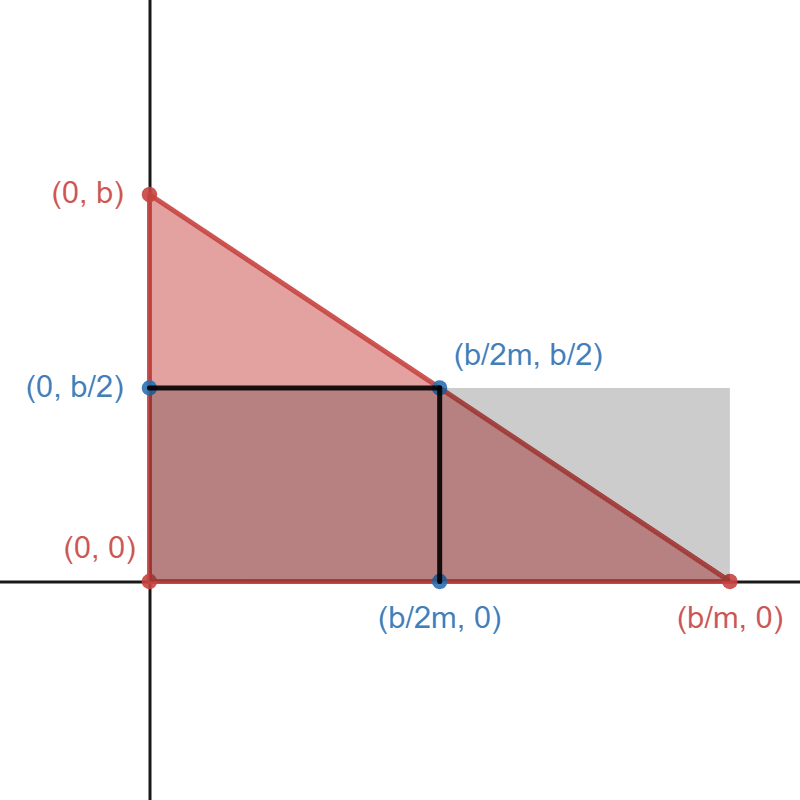
\includegraphics[scale=0.25]{desmos-graph.png}

\raggedright

\begin{minipage}{0.45\textwidth}
 \begin{center}
  Midpoint Approximation
 \end{center}
 For n = 1, $\Delta x$
 \vskip 16pt
 $=\ \dfrac{\dfrac{b}{m}-0}{1}$
 \vskip 16pt
 $=\ \dfrac{b}{m}$ .
 \vskip 16pt
 For midpoint approximation, $\Delta x\, [\, f\,(\, \dfrac{x}{2}\, )\, ]$
 \vskip 16pt
 $=\ \dfrac{b}{m}\, \cdot\, \dfrac{b}{2}$
 \vskip 16pt
 $=\ \dfrac{b^2}{2m}$ .
 \vskip 16pt
 The area obtained from the midpoint approximation equals $\dfrac{b^2}{2m}$ .
\end{minipage}
\hfill
\begin{minipage}{0.45\textwidth}
 \begin{center}
  \vspace{-56mm}
  Triangle
 \end{center}
 \vskip 16pt
 Area of triangle\ $=\dfrac{1}{2}\cdot b\cdot \dfrac{b}{m}$
 \vskip 16pt
 $=\ \dfrac{b^2}{2m}$ .
 \vskip 16pt
 The area of the triangle is $\dfrac{b^2}{2m}$ .
\end{minipage}

\pagebreak

\section{Geometric Argument \# 2}

\begin{large}

 Give a geometric argument to explain why the information from your table showed that $M\, <  \int_{0}^{2} e^{x^2} \, dx\, <\, T$ .

\end{large}

\vspace{1cm}

\begin{minipage}{0.45\textwidth}
 \begin{center}
  Trapezoidal Approximation
  \vskip 16pt
  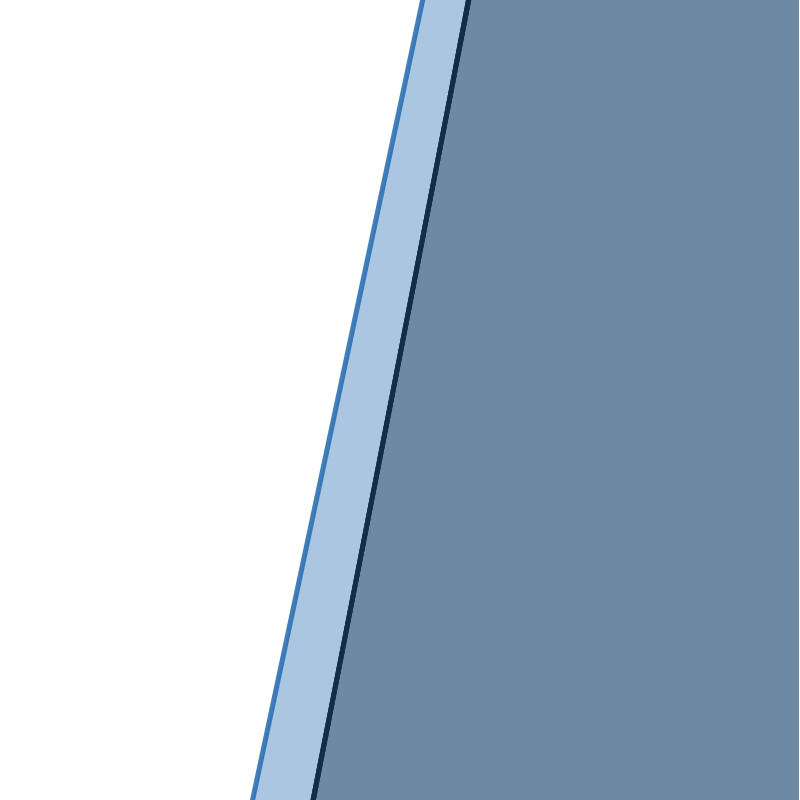
\includegraphics[scale=0.25]{trapezoid.png}
 \end{center}
\end{minipage}
\hfill
\begin{minipage}{0.45\textwidth}
 \begin{center}
  Midpoint Approximation
  \vskip 16pt
  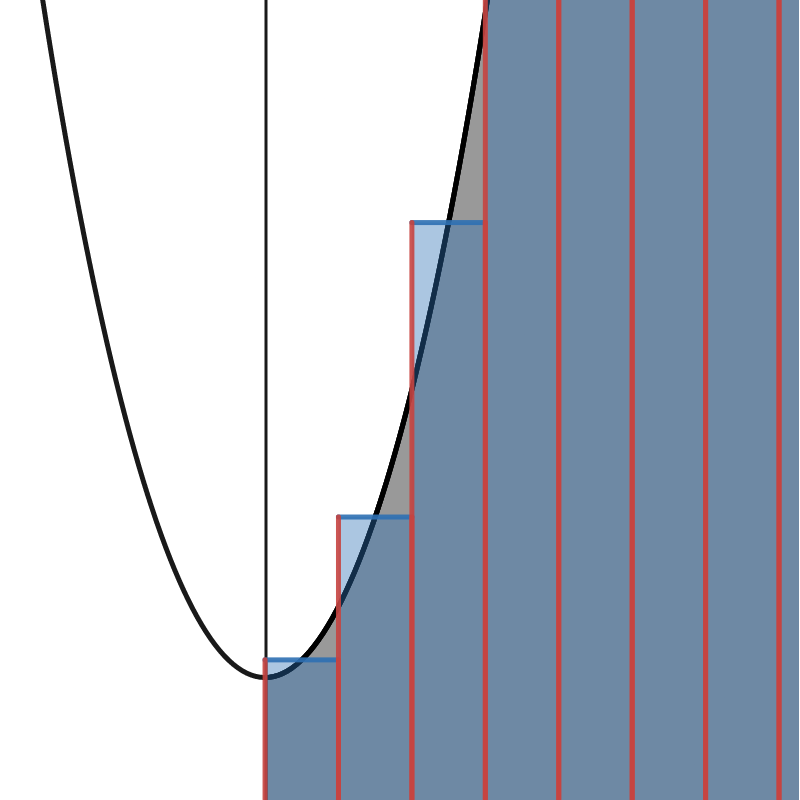
\includegraphics[scale=0.25]{midpoint.png}
 \end{center}
\end{minipage}

\vspace{1cm}

From the two graphs above, it is clear to see that the trapezoidal approximation overestimates the actual area of the function. As for the midpoint approximation, it is a little harder to see that it is an undersestimate. The reason for this is that on the interval [0,2] of the function, it is concave up, leading to these cases being thus.

\pagebreak

\section{Geometric Argument \# 3}

\begin{large}
 Give a geometric argument to explain why the information in your table showed that $T\, <  \int_{1}^{9} \sqrt{x} \, dx\, <\, M$ .
\end{large}

\vspace{1cm}

\begin{minipage}{0.45\textwidth}
 \begin{center}
  Trapezoidal Approximation
  \vskip 16pt
  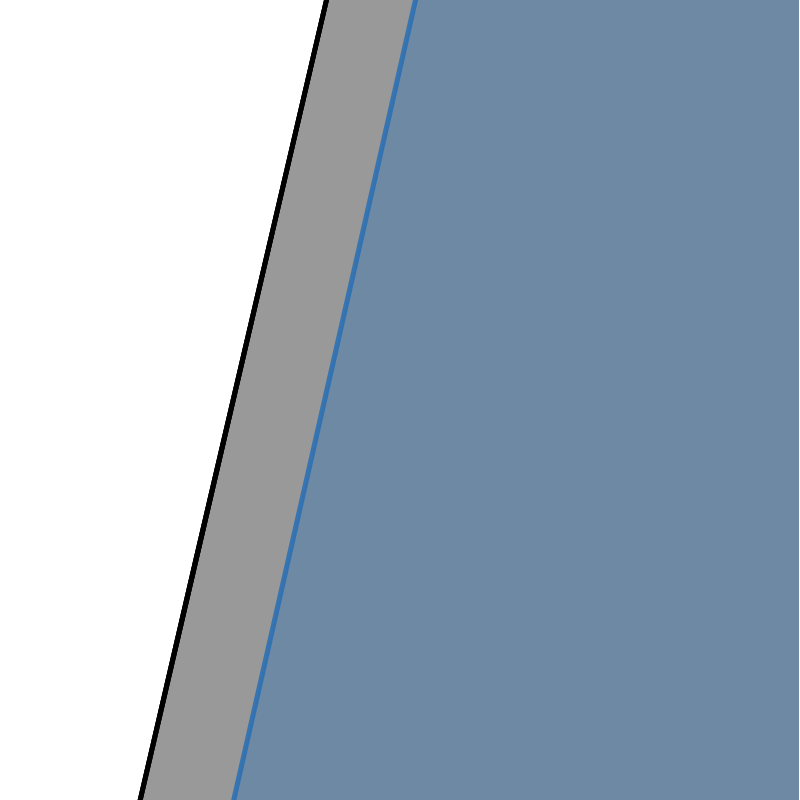
\includegraphics[scale=0.25]{trapezoid1.png}
 \end{center}
\end{minipage}
\hfill
\begin{minipage}{0.45\textwidth}
 \begin{center}
  Midpoint Approximation
  \vskip 16pt
  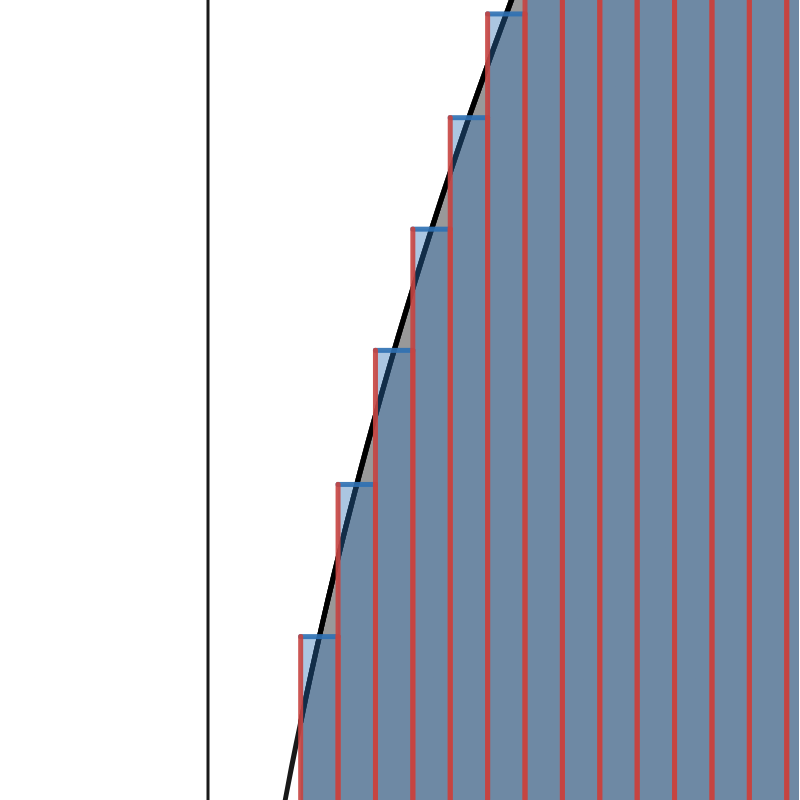
\includegraphics[scale=0.25]{midpoint1.png}
 \end{center}
\end{minipage}

\vspace{1cm}

From the two graphs above, it is clear to see that the trapezoidal approximation underestimates the actual area of the function. As for the midpoint approximation, it is a little harder to see that it is an oversestimate. The reason for this is that on the interval [0,2] of the function, it is concave down, leading to these cases being thus.

\end{document}
